\usecaseristoratore{Visualizzazione notifica nuova prenotazione} 
\label{usecase:Visualizzazione notifica nuova prenotazione}

\begin{figure}[h]
	\centering
	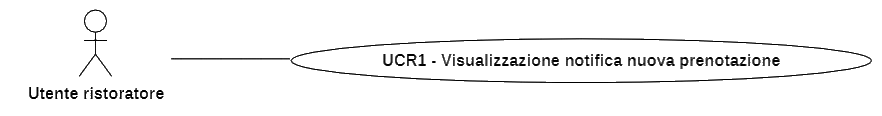
\includegraphics[width=0.9\textwidth]{./uml/UCR1.png} 
	\caption{Visualizzazione notifica nuova prenotazione}
	\label{fig:UCR1}
  \end{figure}

\begin{itemize}
	\item \textbf{Attore principale:} Utente ristoratore.
	
	\item \textbf{Precondizione:} L'Utente base ha confermato la prenotazione ed è tornato alla \textit{Home} (vedi \autoref{usecase:Prenotazione di un tavolo}).

	\item \textbf{Postcondizione:} L'Utente ristoratore visualizza la notifica relativa ad una nuova prenotazione.
     
	\item \textbf{Scenario principale:}
	      \begin{enumerate}
                \item Il Sistema vede che al suo interno è stata fatta una nuova prenotazione;
                \item Il Sistema invia al ristoratore relativo a questa nuova prenotazione una notifica;
                \item L'Utente ristoratore visualizza la notifica relativa ad una nuova prenotazione.
	      \end{enumerate}
\end{itemize}